\chapter{Resultaten} % (fold)
\label{cha:resultaten}
Dit hoofdstuk bevat de resultaten van de verschillende uitgevoerde experimenten. Eerst bespreken we de resultaten van de verschillende uitbreidingen met hun overeenkomstige referentiemodel. Daarna volgt een beschouwing van de invloed van verschillende parameters op de resultaten. Dan komt een kritische vergelijking van de beste modellen met de state-of-the art resultaten. Een laatste set van experimenten vergelijkt CCA en LDA als gids voor de gLSTM-implementatie. Meer specifiek focust de vergelijking op hoe deze twee presteren bij aanwezigheid van ruis in de trainingsdata.

\section{Vergelijking eigen toevoegingen met referenties}  % (fold)
\label{sec:eigen_implementaties}
Zoals vermeld in het vorige hoofdstuk defini\"eren we een referentiemodel getraind met de basisinstellingen voor zowel RNN als LSTM. Deze sectie bespreekt het effect van het toevoegen van LDA aan het RNN-netwerk, het effect van de twee gidsen op het LSTM-netwerk en kort het effect van Gaussnormalisatie bij het beam-search-algoritme op beide netwerken. Er volgt steeds eerst een bespreking van de automatische evaluatie gevolgd door een analyse van de verzamelde statistieken van elk model.

\subsection{RNN}
Zoals al vermeld evalueert Karpathy~\cite{Karpathy2015} de BLEU-score met een Brevity Penalty. Hij voorziet ook geen informatie over Meteor of andere statistieken. Daarom voeren we eerst experimenten uit met de basisinstellingen voor RNN (\emph{ref-RNN}) zonder Brevity Penalty. Hierbij wordt op elk tijdstip de afbeelding aan het netwerk meegegeven. In vergelijking met de uitgevoerde experimenten krijgt het systeem van Karpathy niet op elke tijdstap de afbeelding als invoer. Hij rapporteert dat dit beter presteert. Wanneer de evaluatie toch met Brevity Penalty gebeurt, toont tabel~\ref{table:karpathy_met_bp} dat onze referentie toch zeer sterk overeenkomt met de resultaten van de paper van Karpathy. 

\begin{table}
	\centering
	\begin{tabular}{lllllll}
		& BLEU-1 & BLEU-2 & BLEU-3 & BLEU-4 & Meteor \\ \hline
		RNN (Karpathy~\cite{Karpathy2015})    & 57,3   & 36,9   & 24     & 15,7   & ~           \\    
		ref-RNN + BP     & 55,2   & 36,6   & 23,9   & 15,1   & 14,3          \\
		ref-RNN          & 64,9  & 43,1     & 28,1   & 17,8   & 14,3          \\\hline
	\end{tabular}

	\caption[Resultaten Karpathy in vergelijking met onze referentieresultaten]{Resultaten Karpathy~\cite{Karpathy2015} in vergelijking met onze referentieresultaten}
	\label{table:karpathy_met_bp}
\end{table}

Tabel~\ref{table:rnn_met_lda} toont het effect van het toevoegen van LDA aan de basisimplementatie van RNN. Alle gebruikte metrieken vertonen een stijging. LDA lijkt er dus in te slagen om de semantische drift tegen te gaan.
Figuur~\ref{fig:ldaguide} illustreert met twee voorbeelden hoe LDA het belangrijkste onderwerp terug in de zin krijgt.

In het vorige experiment dient LDA samen met de afbeeldingsrepresentatie op elke tijdstap als invoer van het taalmodel. Experimenten waarbij enkel bij het begin van een zin de afbeelding wordt meegegeven, geven hier tegenover geen verbetering. 

Het toevoegen van Gaussnormalisatie verbetert steeds de score van BLEU-4 en Meteor. Dit zijn de scores die het best overeenkomen met menselijke evaluatie. Net zoals Jia et al.~\cite{Fernando2015} al aanhalen lijkt standaard beam-search lagere BLEU-scores te bevoordelen. Zo domineren de korte zinnen dus niet enkel de gegenereerde zinnen, maar be\"invloeden ze ook de evaluatie.

\begin{table}
	\centering
	\begin{tabular}{lllllll}
		& BLEU-1 & BLEU-2 & BLEU-3 & BLEU-4 & Meteor \\ \hline
		ref-RNN        & 64,9   & 43,1   & 28,1   & 17,8   & 14,3          \\
		RNN + Gauss       & 62,4   & 42     & 28,2   & 18,6   & 16,6          \\
		RNN + LDA         & \textbf{65,4}   & \textbf{44}     & \textbf{29,1}   & 19     & 14,4          \\
		RNN + LDA + Gauss & 62,7   & 42,6   & 28,8   & \textbf{19,5}   & \textbf{16,6}          \\ \hline
	\end{tabular}
	\caption{Vergelijking van de resultaten van RNN na toevoeging LDA en Gaussnormalisatie}	
	\label{table:rnn_met_lda}
\end{table}

\begin{figure}
	\centering
	\begin{minipage}[t]{.3\textwidth}
		\centering
		\vspace{0pt}
		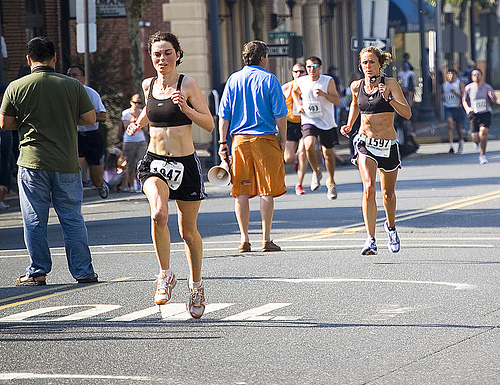
\includegraphics[width=\textwidth]{Images/Results/guide/2}
	\end{minipage}\hfill	
	\begin{minipage}[t]{.7\textwidth}
		\vspace{0pt}
		\begin{tabular}{ll}
			RNN & \texttt{A group of people walking down} \\
		     ~ & \texttt{the street} \\
			RNN+LDA& \texttt{A group of people are running in}\\
			~ & \texttt{the street} \\
		\end{tabular}
	\end{minipage}
	\centering
	\begin{minipage}[t]{.3\textwidth}
		\centering
		\vspace{0pt}
		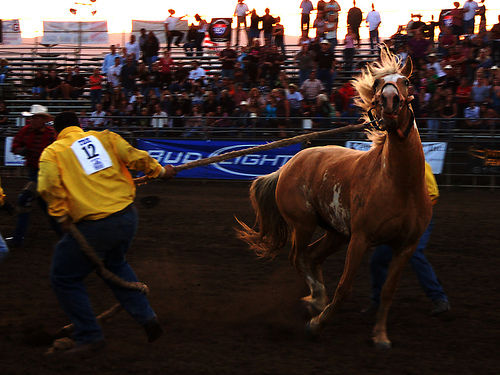
\includegraphics[width=\textwidth]{Images/Results/guide/1}
	\end{minipage}\hfill
	\begin{minipage}[t]{.7\textwidth}
		%\hspace{2pt}
		\vspace{0pt}
		\begin{tabular}{ll}
			RNN & \texttt{A man is standing in front of a crowd} \\
			RNN+LDA & \texttt{A man in a blue shirt is riding}\\
			~ & \texttt{a horse} \\
		\end{tabular}
	\end{minipage}
	\caption{Twee voorbeelden waar LDA de gegenereerde zin verbetert.}
	\label{fig:ldaguide}
\end{figure}

Tabel~\ref{table:rnn_lda_stats} toont de verzamelde statistieken over de gegenereerde zinnen van dezelfde systemen als bij de vorige experimenten. Hierin is \emph{Uniek1} het aantal zinnen dat niet voorkomt in de trainingsverzameling. \emph{Uniek2} is het aantal zinnen dat niet voorkomt in de trainingsverzameling en slechts eenmaal in de verzameling gegenereerde zinnen.
Algemeen valt op dat RNN op een testset van duizend afbeeldingen en een gemiddelde zinslengte van 7 tot 10 woorden slechts een heel beperkte woordenschat leert.
Het toevoegen van LDA vermindert het aantal unieke woorden, maar verhoogt de gemiddelde zinslengte wel lichtjes. Het aantal unieke zinnen van beide types wijzigt niet sterk, al genereert het iets meer vooraf ongeziene zinnen. Het toevoegen van LDA lijkt de creativiteit van de gegenereerde zinnen dus licht te doen dalen.
Het normaliseren met de Gaussiaanse functie bereikt zijn doel. De lengte van de zinnen stijgt met gemiddeld 3 woorden. Toch stijgt het aantal unieke woorden niet mee. De woorden die de normalisatie toevoegt zijn dus veelvoorkomend. Het aantal zinnen dat niet voorkomt in de trainingsset stijgt naar 93\%. Toch is het aantal unieke zinnen van het tweede type niet veel hoger. Het systeem met Gaussnormalisatie genereert met andere woorden veel dezelfde ongeziene zinnen.

\begin{table}
	\centering
	\begin{tabular}{lllll}
		~                 & Unieke woorden & Gem. zinslengte & Uniek1 & Uniek2 \\ \hline
		ref-RNN           & 233            & 7,14           & 785    & 392    \\
		RNN + Gauss       & \textbf{239}   & 10,14          & \textbf{931}    & \textbf{439}    \\
		RNN + LDA         & 189            & 7,59           & 823    & 387    \\
		RNN + LDA + Gauss & 192            & \textbf{10,33}          & 930    & 384    \\\hline
	\end{tabular}
	\caption[Vergelijking van de verzamelde statistieken RNN na toevoeging LDA en Gaussnormalisatie]{Vergelijking van de verzamelde statistieken RNN na toevoeging LDA en Gaussnormalisatie. Hierin is \emph{Uniek1} het aantal zinnen dat niet voorkomt in de trainingsverzameling. \emph{Uniek2} is het aantal zinnen dat niet voorkomt in de trainingsverzameling en slechts \'e\'en keer wordt gegenereerd.}
	\label{table:rnn_lda_stats}
\end{table}

\subsection{LSTM}
Rechtstreeks vergelijken met de LSTM-implementatie van Vinyals~\cite{Google} is onmogelijk. Hij gebruikt niet alleen een ander CNN, maar gebruikt bovendien ook ensemble-methodes wat te veel tijd kost voor onze implementatie. Daarom bepalen we ook hier met de standaardinstellingen een referentiemodel (\emph{ref-LSTM}). Tabel~\ref{table:lstm_results} vergelijkt de resultaten van de originele paper, het referentiemodel en de gLSTM's. De experimenten bevatten resultaten voor LDA met 120 onderwerpen, CCA met een multimodale voorstelling van grootte 256 en opnieuw het effect van Gaussnormalisatie. Ook hier toont de tabel dat de referentiewaarden ondanks een eenvoudiger model toch dicht aanleunen bij de originele resultaten. 

Zowel het gebruik van LDA als CCA als gids in het gLSTM-netwerk verbetert de resultaten op elke metriek ten opzichte van de referentie. Daarenboven presteren beide gLSTM-netwerken beter dan de originele paper op elke metriek behalve BLEU-1. Dit effect is het grootste voor CCA, op de Meteor-score na. Appendix~\ref{app:generalResults} toont een aantal afbeeldingen met bijbehorende gegenereerde zin als voorbeeld. Voor zowel het referentiemodel als gLSTM met LDA zorgt Gaussnormalisatie voor een aanzienlijke verbetering voor BLEU-3, BLEU-4 en Meteor. Deze scores komen bovendien het meest overeen met menselijke evaluatie. Bij gLSTM met CCA doet er zich een vreemd fenomeen voor en verslechtert de normalisatie de BLEU-scores, maar verbetert ze de Meteor-score. 
Het effect van LDA met Gauss en CCA ligt dicht bij elkaar. Toch scoort LDA met Gauss op de scores die meer correleren met menselijke evaluatie nipt het beste.
    \begin{table}
    	\centering
    	\begin{tabular}{llllll}
    		~                   & BLEU-1 & BLEU-2 & BLEU-3 & BLEU-4 & Meteor \\ \hline
    		LSTM (Vinyals~\cite{Google})      & \textbf{66,3}   & 42,3   & 27,7   & 18,3   & ~     \\ 
    		ref-LSTM         & 62,1   & 41,4   & 27,1   & 17,6   & 15,1  \\
    		LSTM+Gauss        & 61,2   & 41,1   & 27,3   & 18,2   & 16,9  \\
    		gLSTM+LDA         & 64,4   & 43,2   & 28,1   & 17,8   & 16  \\
    		gLSTM+LDA+Gauss & 62,7   & 42,5   & 28,8   & \textbf{19,4}   & \textbf{17,4}  \\
	        gLSTM+CCA         & 63,7   & \textbf{43,4}   & \textbf{29,2}   &19,3   & 15,8  \\
	        gLSTM+CCA+Gauss & 62,1   & 41,9   & 28,2   & 18,7   & 17,2  \\\hline
    	\end{tabular}
   	\caption{Vergelijking van de resultaten LSTM met twee gidsen en met Gaussnormalisatie}	
   	\label{table:lstm_results}
    \end{table}

Tabel~\ref{table:lstm_stats} toont de verzamelde statistieken over de gegenereerde zinnen van de vorige systemen. In vergelijking met het referentie-RNN leert het LSTM-netwerk een groter vocabularium (ongeveer 40\% groter). Ook de zinnen zijn gemiddeld iets langer. Het aantal unieke zinnen van het eerste type daalt licht, maar het aantal van het tweede type is gelijkaardig.
Ook hier is het effect van Gaussnormalisatie hetzelfde. De gemiddelde zinslengte stijgt gevoelig en ook het aantal unieke zinnen van type 1 stijgt fel. Het aantal volledig unieke zinnen (\emph{Uniek2}) van beide gLSTM's stijgt sterk door het toevoegen van Gaussnormalisatie tot 60\% voor CCA. CCA als gids leert ook meer unieke woorden dan LDA en lijkt dus tot iets creatievere zinnen te leiden.
    \begin{table}
    	\centering
    	\begin{tabular}{llllll}
    		~                   & Unieke woorden & Gem. zinslengte & Uniek1 & Uniek2 \\ \hline
    		ref-LSTM         				  & 327   & 7,89   & 723   & 399  \\
    		LSTM+Gauss        				  & 351   & 10,36   & 905   & 437  \\
    		gLSTM+LDA         				  & 296   & 8,33   & 775   & 490     \\
    		gLSTM+LDA+Gauss 				  & 323   & \textbf{10,43}   & 907   & 541     \\
    		gLSTM+CCA         				  & 347   & 7,96   & 775   &557   \\
    		gLSTM+CCA+Gauss 				  & \textbf{383}   & 10,36   & \textbf{915}   & \textbf{602}    \\\hline
    	\end{tabular}
	\caption[Vergelijking van de verzamelde statistieken LSTM na toevoeging LDA, CCA en Gaussnormalisatie]{Vergelijking van de verzamelde statistieken LSTM na toevoeging LDA, CCA en Gaussnormalisatie. Hierin is \emph{Uniek1} het aantal zinnen dat niet voorkomt in de trainingsverzameling. \emph{Uniek2} is het aantal zinnen dat niet voorkomt in de trainingsverzameling en slechts \'e\'en keer wordt gegenereerd.}
    	\label{table:lstm_stats}
    \end{table}
    
\subsection{Problemen met de ontwikkelde systemen}
De best presterende systemen in deze masterproef zijn niet altijd in staat om perfect de afbeeldingen te beschrijven.
 De gegenereerde zinnen zijn wel altijd vloeiend en grammaticaal correct.
  Figuren~\ref{fig:intermediateresult}~en~\ref{fig:badresults} in de appendix geven hiervan een aantal voorbeelden.
Vaak voorkomende problemen zijn de incorrecte toewijzing van kleuren aan objecten.
Een tweede type van problemen doet zich voor wanneer het systeem concrete aantallen voorspelt.
Dikwijls verkiest het systeem het woord \texttt{two} terwijl er meer dan twee objecten in de afbeelding staan.
LDA biedt hier zeker geen hulp, aangezien er een onderwerp met aantallen bestaat waarin \texttt{two} het meest waarschijnlijke woord is.

Naast deze frequente problemen is er ook een beperkt aantal zinnen waar het systeem geen zicht krijgt op wat er op de afbeelding staat.
Deze afbeeldingen komen vaak overeen met de afbeeldingen waar het LDA-netwerk ook geen correcte onderwerpverdeling bepaalt.
De verklaring hiervoor ligt wellicht in slechte representaties gemaakt door het gebruikte CNN.
    
\section{Invloed van parameters}
\label{sec:invloed-parameters}
Deze sectie bekijkt de invloed van de waarde van enkele parameters die in de voorgaande experimenten hetzelfde bleven. Als eerste volgt een analyse van het effect van de gebruikte beam-lengte. Vervolgens volgt een korte bespreking van het aantal onderwerpen van LDA. Hierna experimenteren we met de gebruikte grootte van de CCA-projectie. Als laatste bekijken we de gevolgen van de ge\"implementeerde normalisatiemethodes.

\subsection{Beam-lengte}
De gekozen beam-lengte bij het beam-search-algoritme speelt een rol in de uitvoeringstijd en resultaten van elk systeem. 
Een grotere beam-lengte zorgt ervoor dat het zoekalgoritme veel meer mogelijkheden onderzoekt en bijgevolg meer tijd nodig heeft om zinnen te genereren.
Ideaal gezien bekijkt het systeem alle mogelijke zinnen, wat neerkomt op een beam-lengte ter grootte van het vocabularium, maar dit is praktisch niet haalbaar door de te hoge vereiste tijd.
Om die reden bekijkt dit onderdeel in welke mate de beam-lengte de resultaten be\"invloedt.
Tabel~\ref{table:beam} toont resultaten voor een gLSTM-model met als gids een LDA-vector met 120 onderwerpen. De beam-grootte varieert tussen 1 en 100. Voor waarden groter dan 100 duurt de generatie te lang voor praktische toepassingen. Tabel~\ref{table:beam_gauss} toont hetzelfde type van experimenten maar deze keer ook met Gaussnormalisatie. Uit deze resultaten blijkt dat een beam-grootte van 1, wat overeenkomt met steeds het meest waarschijnlijke woord nemen, de slechtste scores oplevert. Uit de hogere beam-groottes kan geen eenduidige conclusie worden getrokken. Zonder Gaussnormalisatie presteert een grootte van 75 het beste op BLEU-1 tot BLEU-3, maar niet op de belangrijke BLEU-4-score. Met Gaussnormalisatie scoort een grootte van 25 de beste resultaten. Een algemene beam-grootte van 50 zoals de standaard in deze thesis, lijkt dus een acceptabel compromis tussen deze twee best presterende groottes.

    \begin{table}
    	\centering
    	\begin{tabular}{lllll}
    		Beam-grootte                   & BLEU-1 & BLEU-2 & BLEU-3 & BLEU-4  \\ \hline
	    	1	      & 57,9   & 39,1   & 25,5   & 16,3        \\ 
    		5         & 62,6   & 42,6   & 28,3   & \textbf{18,6}     \\
    		10         & 63,6   & 42,9   & 28,4   & 18,5    \\
    		25        & 64,4   & 43,3   & 28,4   & 18,4     \\
    		50		  & 64,4   & 43,2   & 28,1   & 17,8    \\
    		75        & \textbf{64,9}   & \textbf{43,7}   & \textbf{29,5}   & 18,2    \\
    	    100		  & 64,7   & 43,4   & 28,2   & 17,9     \\\hline
    	\end{tabular}
    	\caption{Vergelijking van de BLEU-resultaten van gLSTM met verschillende beam-groottes en als gids LDA met 120 onderwerpen.}	
    	\label{table:beam}
    \end{table}

    \begin{table}
    	\centering
    	\begin{tabular}{lllll}
    		Beam-grootte & BLEU-1 & BLEU-2 & BLEU-3 & BLEU-4  \\ \hline
    		1	      & 57,9   & 39,1   & 25,5   & 16,3        \\ 
    		5         & 62,1   & 42,4   & 28,6   & 19,1     \\
    		10        & 62,9   & 42,8   & 28,8   & 19,2    \\
    		25        & \textbf{62,9}   & \textbf{43,7}   & \textbf{28,9}   & \textbf{19,4}     \\
    		50		  & 62,7   & 43,5   & 28,8   & \textbf{19,4}    \\
    		75        & 62,5   & 42,2   & 28,5   & 19,2    \\ \hline
    	\end{tabular}
    	\caption{Vergelijking van de BLEU-resultaten van gLSTM met Gaussnormalisatie en verschillende beam-groottes en als gids LDA met 120 onderwerpen.}	
    	\label{table:beam_gauss}
    \end{table}

\subsection{Aantal onderwerpen LDA}
Tijdens het leren van LDA is er, buiten de manuele inspectie van de kansverdeling van de woorden bij elk onderwerp, geen concrete aanwijzing of een bepaald aantal onderwerpen leidt tot betere verdelingen.
Tijdens het trainen van het neuraal netwerk geeft de fout op de validatieverzameling wel een indicatie van hoe goed het netwerk die verdelingen kan voorspellen op basis van een afbeelding.
Na dit trainen gebruikt het gLSTM-netwerk deze verdelingen als gids bij het genereren van de zinnen.
In deze drie stappen speelt het aantal onderwerpen dus steeds een rol, maar het is finaal niet duidelijk wat het ideale aantal precies is.
De paper van Jin et al.~\cite{Jin2015} die ook de LDA-onderwerpverdeling als extra invoer in het LSTM-netwerk voert, gebruikt 80 onderwerpen.
Daarom beschouwen de experimenten aantallen rond deze 80. Na manuele inspectie van de woordverdelingen per onderwerp bleek 50 onderwerpen weinig duidelijk te onderscheiden onderwerpen af te leiden.
Tabel~\ref{table:lda-onderwerpen} bevat daarom enkel resultaten voor 80, 100 en 120 onderwerpen.

    \begin{table}
    	\centering
    	\begin{tabular}{lllllll}
    		~                 &\#onderw.  & BLEU-1 & BLEU-2 & BLEU-3 & BLEU-4 & Meteor \\ \hline
    		gLSTM+LDA       & 80  & 61,4   & 40,4  & 26   & 16,7   & 14,7     \\ 
    		gLSTM+LDA      & 100  & \textbf{64,4}   & \textbf{43,3}   & \textbf{28,6}   & \textbf{18,6}   & 15,9  \\
    		gLSTM+LDA      &120   & \textbf{64,4}   & 43,2   & 28,1   & 17,8   & \textbf{16}  \\\hline
    		gLSTM+LDA+Gauss &80 & \textbf{65}   & \textbf{43,5}   & 28,4   & 18,2   & 16,2  \\ 
    		gLSTM+LDA+Gauss& 100&62,5& 42,1   & 28,2   & 18,9   & 17,2    \\
    	gLSTM+LDA+Gauss&120 & 62,7   & 42,5   &\textbf{28,8}   & \textbf{19,4}   & \textbf{17,4}  \\\hline
    	\end{tabular}
    	\caption{Vergelijking van de resultaten gLSTM met LDA als gids en variabel aantal onderwerpen}	
    	\label{table:lda-onderwerpen}
    \end{table}
    
Uit de resultaten blijkt dat zonder Gaussnormalisatie LDA met 100 onderwerpen het beste scoort op BLEU en ongeveer even goed als 120 op Meteor. 80 onderwerpen lijkt te weinig om het gLSTM-netwerk voldoende bij te sturen. Na toevoeging van Gaussnormalisatie presteren 120 onderwerpen beter op de belangrijkste evaluatiecriteria. Een mogelijke verklaring voor dit gedrag ligt in het feit dat Gaussnormalisatie zorgt voor langere zinnen. De laatste woorden in deze zinnen hebben bijgevolg meer last van semantische drift. Hier speelt LDA als semantische gids dus een belangrijkere rol. Het blijkt dus dat een grotere vector voor LDA vooral voor lange zinnen een meerwaarde biedt. Er bestaat wel een bovengrens in de grootte. Wanneer het aantal onderwerpen te hoog wordt, is het LDA-algoritme niet langer in staat om zinnige onderwerpen te ontdekken.

\subsection{Vectorgrootte CCA} 
Het CCA-algoritme laat toe om het aantal correlatiecomponenten te kiezen. De invloed van dit aantal op de afbeeldingsgeneratie is niet meteen duidelijk. Daarom beschouwen we net zoals Jia et al.~\cite{Fernando2015} eerst een grootte van 256, maar bekijken ook de resultaten voor een grootte van 128 en 512. De tijd nodig voor het trainen van het gLSTM-netwerk stijgt sterk met de gekozen gidsgrootte. Dit maakt een afweging tussen grootte en trainingstijd misschien noodzakelijk.

Tabel~\ref{table:results_cca} toont de resultaten van de automatische evaluatiemethodes voor de drie types. Het is duidelijk dat CCA met een vectorgrootte van 256 het beste presteert op alle evaluatiemethodes. Dit model genereert eveneens meer unieke woorden en meer unieke zinnen van beide types. Een mogelijke verklaring hiervoor is dat CCA met een grootte van 128 te weinig semantische informatie meegeeft. Bij CCA met een hogere vectorgrootte bevat de vector bij elke toevoeging steeds minder belangrijke informatie. Wanneer de vector dus te groot wordt, gaat de minder belangrijke informatie zwaarder doorwegen en de resultaten bijgevolg verminderen.

Het fenomeen dat de grootte meer speelt in combinatie met Gaussnormalisatie zoals bij LDA was hier niet zichtbaar. Een mogelijke verklaring hiervoor is dat CCA als gids zonder Gaussnormalisatie al zeer goede prestaties bereikt.
\begin{table}
	\centering
	\begin{tabular}{lllllll}
		~              & CCA-grootte     & BLEU-1 & BLEU-2 & BLEU-3 & BLEU-4 & Meteor \\ \hline
		gLSTM+CCA & 128        & 63,5   & 42,5 			& 27,9   & 18   & 15,5  \\
		gLSTM+CCA & 256        & \textbf{63,7}   & \textbf{43,4}   & \textbf{29,2}   & \textbf{19,3}   & \textbf{15,8}  \\
		gLSTM+CCA & 512        & 63,3   & 42,2   & 28,2   & 18,3 & 15,1  \\ \hline
	
	\end{tabular}

	\caption{Automatische evaluatieresultaten voor verschillend aantal correlatiecomponenten CCA}
		\label{table:results_cca}
\end{table}



\subsection{Effect verschillende normalisatiemethodes}
Deze thesis maakt gebruik van drie verschillende normalisatiemethodes. Als eerste zijn er Gauss en Min-Hinge met als doel de lengte van de zinnen te verhogen en zo ook hun automatische evaluatie te verbeteren. Als derde introduceert deze masterproef de idf-gewogen normalisatiefunctie. Deze heeft als doel de creativiteit van de zinnen te verhogen om zo minder algemene beschrijvingen te genereren.

\subsubsection{Gaussnormalisatie}
In de paper van Jia et al.~\cite{Fernando2015} presteert Gaussnormalisatie voor de meeste metrieken veruit het beste. 
Dit is ook het geval bij de in deze masterproef bestudeerde normalisatiefuncties. Gaussnormalisatie verhoogt vrijwel steeds de BLEU-3-, BLEU-4- en Meteor-score. De lagere BLEU-scores (zeker zonder Brevity Penalty) lijken een voorkeur te hebben voor korte zinnen. Op de belangrijkere scores zorgt Gaussnormalisatie voor verbetering ten opzichte van een ongenormaliseerd systeem. De Brevity Penalty na Gaussnormalisatie is bovendien steeds gelijk aan 1, waardoor de scores met of zonder BP dezelfde zijn.
Het tweede doel is het genereren van langere zinnen door de lengteverdeling van de trainingsverzameling na te bootsen.
In alle bestudeerde configuraties slaagt de normalisatie erin om de lengte van gemiddeld 7,5 te doen stijgen naar 10,3 woorden per zin. Figuur~\ref{fig:gauss} toont voor het standaard RNN-systeem hoe de lengteverdeling wijzigt. Deze stijging gaat gepaard met een sterke toename van de zinnen die niet voorkomen in de trainingsset tot meer dan 90\%. Het aantal unieke zinnen van het tweede type verhoogt slechts licht. 

Een ander interessant fenomeen vertoont zich in de frequentie van de gebruikte woorden. Ondanks de stijging van het aantal woorden bij het gebruik van Gaussnormalisatie, vertonen de meest gebruikte woorden deze stijging niet en blijven de aantallen zelfs exact dezelfde. Een mogelijke verklaring ligt in de manier waarop het systeem zinnen genereert. Vermoedelijk zijn de zinnen vrijwel hetzelfde, maar zorgt de Gaussnormalisatie ervoor dat het achteraan de zin nog extra informatie over de afbeelding toevoegt. Dit kan ook een verklaring zijn voor de toename in creativiteit. De informatie aan het einde is heel variabel, terwijl de algemene en vaak iets vagere informatie aan het begin van de zin vaak gelijkaardig is. Een groot deel van de zinnen begint bijvoorbeeld met de woorden \texttt{A man is}, die tevens in elke configuratie bij de vijf meest voorkomende woorden horen. Figuur~\ref{fig:gauss_improve} toont twee voorbeelden waar Gaussnormalisatie zorgt voor een meer volledige beschrijving.

\begin{figure}[tb]
	\centering
	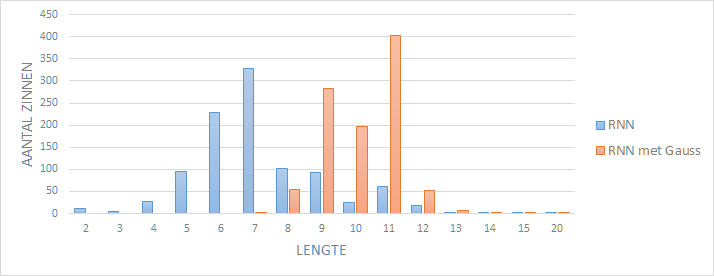
\includegraphics[width=\textwidth]{Images/gauss_length.PNG}
	\caption[Effect van Gaussnormalisatie op de zinslengteverdeling]{Effect van Gaussnormalisatie op de zinslengteverdeling voor het standaard RNN-systeem.}
	\label{fig:gauss}
\end{figure}  
\begin{figure}
	\centering
	\begin{minipage}[t]{.3\textwidth}
		\centering
		\vspace{0pt}
		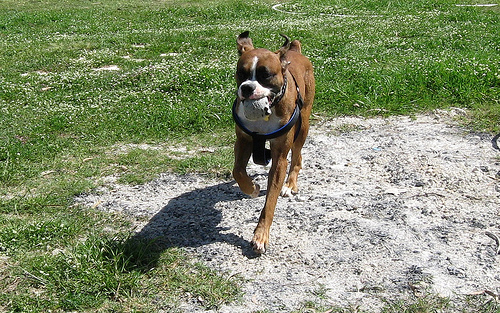
\includegraphics[width=\textwidth]{Images/Results/gauss/hond}
	\end{minipage}\hfill	
	\begin{minipage}[t]{.7\textwidth}
		\vspace{0pt}
		\begin{tabular}{ll}
			Standaard & \texttt{A dog runs through the grass} \\
			Met Gauss & \texttt{A brown and white dog is}\\
			~ & \texttt{running through the grass} \\
		\end{tabular}
	\end{minipage}
			\centering
		\begin{minipage}[t]{.3\textwidth}
			\centering
			\vspace{0pt}
			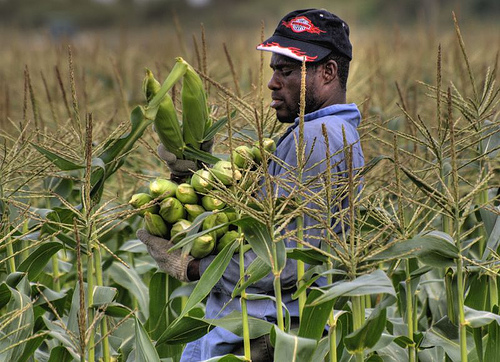
\includegraphics[width=\textwidth]{Images/Results/gauss/man}
		\end{minipage}\hfill
		\begin{minipage}[t]{.7\textwidth}
			\vspace{0pt}
			\begin{tabular}{ll}
				Standaard & \texttt{A man in a green shirt is holding a tree} \\
				Met Gauss & \texttt{A man in a blue shirt is standing }\\
				~ & \texttt{in a field} \\
			\end{tabular}
		\end{minipage}
\caption{Twee voorbeelden waar Gaussnormalisatie de gegenereerde zin verbetert.}
\label{fig:gauss_improve}
\end{figure}
\subsubsection{Min-hinge-normalisatie}
Net als Gaussnormalisatie tracht ook min-hinge-normalisatie langere zinnen te genereren.
Na experimenten met hetzelfde gLSTM-netwerk met als gids CCA met een vectorgrootte van 128, blijkt dat de min-hinge-normalisatie hier niet in slaagt. Daarnaast verslechtert het bovendien de resultaten. Om die redenen zijn geen verdere experimenten met deze vorm van normalisatie uitgevoerd. Tabel~\ref{table:minhinge} toont de vergelijking van een ongenormaliseerd systeem, Gaussnormalisatie en min-hinge-normalisatie.

\begin{table}
	\centering
	\begin{tabular}{lllllll}
		~                  & BLEU-1 & BLEU-2 & BLEU-3 & BLEU-4 & Meteor&Zinslengte \\ \hline
		gLSTM        & 63,5   & 42,5 			& 27,9   & 18   & 15,5&7,99  \\
		gLSTM+min-hfinge & 60,4   &40,4    &26,8   & 17,6   & 15,5& 7,98 \\
		gLSTM+Gauss   & 62,1   & 41,9   & 28,2   & 18,3 & 15,1& 10,54 \\ \hline
		
	\end{tabular}
	
	\caption{Automatische evaluatieresultaten voor hetzelfde gLSTM-netwerk met als gids CCA met vectorgrootte 128 en verschillende normalisatiemethodes}
	\label{table:minhinge}
\end{table}

\subsubsection{Idf-normalisatie}
Als laatste vorm introduceren we idf-normalisatie. Hierbij is het doel om langere zinnen te genereren die bovendien creatiever zijn.
Dit is een reactie op de observatie dat slechts hoogstens de helft van de zinnen echt uniek zijn. Bovendien is de woordenschat van de getrainde modellen steeds beperkt tot
maximaal 383 woorden terwijl het vocabularium van de trainingsset 7413 verschillende woorden bevat.
Het is te verwachten dat door het aanmoedigen van minder frequente woorden de BLEU-score daalt. Omdat Meteor wel rekening houdt met synoniemen, voorspellen we een minder sterke daling dan bij BLEU.

De experimenten vergelijken gLSTM met LDA met 120 onderwerpen als gids, met en zonder idf-normalisatie.
Tabel \ref{table:idf-results} bevat de resultaten van de automatische evaluatie. Het is duidelijk dat de BLEU-score dramatisch daalt. Ook de Meteor-score daalt, maar de daling is zoals verwacht minder sterk.

Tabel~\ref{table:idf-stats} toont dat idf-normalisatie het doel wel bereikt. De gemiddelde lengte verhoogt tot ongeveer het niveau van Gaussnormalisatie. 99\% van de gegenereerde zinnen komt niet voor in de trainingsverzameling. 93\% van de zinnen komt slechts \'e\'en keer voor in de trainingsverzameling en gegenereerde zinnen samen. Het is dus duidelijk dat de creativiteit van dit systeem een stuk hoger ligt dan zonder idf-normalisatie.
\begin{table}
	\centering
	\begin{tabular}{llllll}
		~                  & BLEU-1 & BLEU-2 & BLEU-3 & BLEU-4 & Meteor \\ \hline
		gLSTM        & 64,4   & 43,2 			& 28,1   & 17,8   & 16 \\
		gLSTM+idf   & 40,7   & 23,2   & 13,4   & 7,6 & 12,82 \\ \hline
		
	\end{tabular}
	
	\caption{Vergelijking van automatische evaluatieresultaten voor hetzelfde gLSTM-netwerk met als gids LDA met 120 onderwerpen met en zonder idf-normalisatie}
	\label{table:idf-results}
\end{table}

    \begin{table}
    	\centering
    	\begin{tabular}{llllll}
    		~                   & Unieke woorden & Gem. zinslengte & Uniek1 & Uniek2 \\ \hline
    		gLSTM         				  & 296   & 8,33   & 775   & 490  \\
    		
    		gLSTM+idf 				  & \textbf{721}   & \textbf{10,54}   & \textbf{991}   & \textbf{927}    \\\hline
    	\end{tabular}
    	\caption[Vergelijking effect idf-normalisatie op de statistieken van gLSTM met LDA met 120 onderwerpen]{Vergelijking van het effect van idf-normalisatie op de statistieken van gLSTM met LDA met 120 onderwerpen. Hierin is \emph{Uniek1} het aantal zinnen dat niet voorkomt in de trainingsverzameling. \emph{Uniek2} is het aantal zinnen dat niet voorkomt in de trainingsverzameling en slechts \'e\'en keer wordt gegenereerd.}
    	\label{table:idf-stats}
    \end{table}
    
Met een manuele kwalitatieve evaluatie van de gegenereerde zinnen brengen we in kaart of deze creativiteit sterk ten koste gaat van de zinskwaliteit zoals de BLEU- en Meteorscores suggereren. 
De meeste afbeeldingen in de testverzameling genereren zowel correcte grammaticaal als inhoudelijk juiste zinnen.
Daarnaast is het woordgebruik duidelijk veel gevarieerder en vloeiender.
Figuur~\ref{fig:betteridf} toont een aantal voorbeelden waarbij idf-normalisatie voor verbetering zorgt.
Helaas gaat het systeem bij het genereren van veel zinnen duidelijk in de mist. Een vaak voorkomend probleem zijn woordherhalingen. Ook de woorden \texttt{African American} komen te vaak voor bij beschrijvingen waar mensen in voorkomen. Dit kan deels verklaard worden doordat de woorden \texttt{African} en \texttt{American} in hetzelfde onderwerp voorkomen als \texttt{white}, maar nu de voorkeur krijgen omdat ze weinig voorkomen in de trainingsverzameling. Voorbeelden van foutief gegenereerde zinnen zijn:\\
\texttt{african american african american male is sitting on a rock ledge}\\
\texttt{lone lone lone lone lone lone lone skier splashes in the water}

\begin{figure}
	\centering
	\begin{minipage}[t]{.3\textwidth}
		\centering
		\vspace{0pt}
		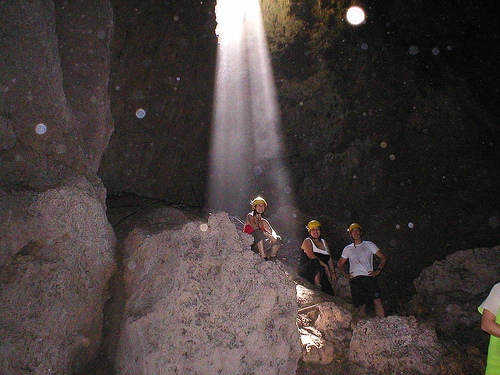
\includegraphics[width=\textwidth]{Images/Results/idf/rock}
	\end{minipage}\hfill	
	\begin{minipage}[t]{.7\textwidth}
		\vspace{0pt}
		\begin{tabular}{ll}
			gLSTM & \texttt{a group of people are standing } \\
			~ & \texttt{in the woods} \\
			gLSTM+idf & \texttt{several people are standing}\\
			~ & \texttt{near a large rock formation} \\
		\end{tabular}
	\end{minipage}
	\centering
	\begin{minipage}[t]{.3\textwidth}
		\centering
		\vspace{0pt}
		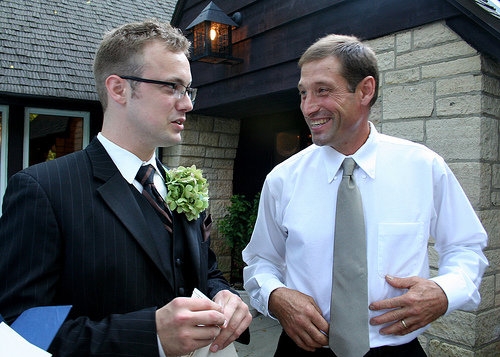
\includegraphics[width=\textwidth]{Images/Results/idf/trouw}
	\end{minipage}\hfill
	\begin{minipage}[t]{.7\textwidth}
		\vspace{0pt}
		\begin{tabular}{ll}
			gLSTM & \texttt{A man and woman are talking} \\ 
			~ & \texttt{to each other} \\
			gLSTM+idf & \texttt{Two men dressed in formal attire}\\
			~ & \texttt{share a conversation} \\
		\end{tabular}
	\end{minipage}
	\caption{Twee voorbeelden waar idf-normalisatie de gegenereerde zin verbetert.}
	\label{fig:betteridf}
\end{figure}

Deze vorm van normalisatie lijkt in vele gevallen creatievere, minder vage en soms menselijkere zinnen te genereren. Toch bevat het nog een groot aantal storende fouten. Verder onderzoek naar dit type normalisatie, misschien in combinatie met bijvoorbeeld Gaussnormalisatie, lijkt nuttig. 

\section{Vergelijking met literatuur} % (fold)
\label{sec:vergelijking_met_literatuur}
Na de grondige evaluatie van de eigen resultaten volgt in dit onderdeel een vergelijking met de resultaten uit de meest recente literatuur.
Deze vergelijking bevat onder andere het werk van Vinyals et al.~\cite{Google} dat de basis vormt voor het LSTM-netwerk in deze masterproef. 
De vergelijking bevat ook de paper van Jia et al.~\cite{Fernando2015} die als eerste gLSTM's voorstelden.
Naast deze twee hoog scorende papers bestaan er nog twee systemen die allebei aandacht integreren in hun model~\cite{Jin2015,Xu2015}.
Jin et al.~\cite{Jin2015} voegen bovendien een sc\`enevector op basis van LDA toe aan het gebruikte LSTM-netwerk.
Tabel~\ref{table:sota} biedt een overzicht van de best presterende eigen modellen in vergelijking met de beste modellen uit de literatuur.
Algemeen is duidelijk dat de best presterende modellen uit deze masterproef op de laatste paper na zeker in de buurt komen van de state-of-the-art resultaten.

De experimenten van dit werk gebruiken een aantal ongewijzigde parameters.
Deze keuze is gemaakt omdat het trainen van een netwerk met een bepaalde instelling steeds bijzonder veel tijd vraagt.
Zo duurt het trainen van een netwerk met RNN ongeveer vijf dagen op de gebruikte hardware, terwijl een netwerk met LSTM ongeveer acht dagen vraagt.
Een betere afstelling van deze parameters maakt betere resultaten van dezelfde systemen mogelijk.
Dit is een mogelijke verklaring waarom het gLSTM-netwerk van Jia met 256 als vectorgrootte voor CCA en Gaussnormalisatie beter scoort dan onze implementatie.
Toch komen de resultaten van deze masterproef zeker in de buurt.

Beide aandachtsmodellen scoren het beste in de literatuur. Het toevoegen van aandacht aan de netwerken van deze masterproef lijkt dus een veelbelovende uitbreiding.
Het model van \cite{Jin2015} claimt de hoogste resultaten op de Flickr30k testverzameling.
Het toevoegen van aandacht aan het netwerk maakt wel duidelijk het trainen van het netwerk complexer en bijgevolg ook trager.
Het \emph{RNN+LDA}-model doet daarom zeker niet onder. De resultaten liggen immers niet veraf en door het gebruik van een RNN en weinig complexe toevoegingen traint en voorspelt het sneller.
In vergelijking met ons model bestaande uit gLSTM met LDA gebruiken Jin et al.~\cite{Jin2015} bijvoorbeeld een complexere CNN die aparte regio's ontdekt. De ontdekte regio's en hun representatie vormen samen de voorstelling van een afbeelding in plaats van \'e\'en CNN-output zoals in deze thesis. Daarnaast maakt hun werk gebruik van twee LSTM's met elk een andere functie. Het systeem integreert bovendien een aandachtsmodel in het netwerk.
Het is wel opvallend dat deze best scorende paper werd geschreven in juni 2015, maar tot op heden nog geen publicatie heeft.

In de experimenten van Jin et al.~\cite{Jin2015} bepalen ze hun vocabularium door enkel woorden te selecteren die meer dan 20 keer voorkomen, wat hoger is dan de 5 in dit werk waardoor het systeem minder woorden moet leren begrijpen. Het effect van dit aantal woorden vormt dus ook een interessante te bestuderen parameter.

\begin{table}
	\centering
	\begin{tabular}{llllll}
		~                  & BLEU-1 & BLEU-2 & BLEU-3 & BLEU-4 & Meteor \\ \hline
		RNN+LDA            & \textbf{65,4}   & \textbf{44}     & 29,1   & 19     & 14,38  \\
		RNN+LDA+Gauss      & 62,7   & 42,6   & 28,8   & \textbf{19,5}   & 16,62  \\
		gLSTM+LDA+Gauss    & 62,7   & 42,5   & 28,8   & 19,4   & \textbf{17,4}   \\
		gLSTM+CCA          & 63,7   & 43,4   & \textbf{29,2}   & 19,3   & 15,76  \\
		gLSTM+CCA+Gauss    & 62,1   & 41,9   & 28,2   & 18,7   & 17,18  \\ \hline
		
		Google NIC~\cite{Google}           & 66,3   & 42,3   & 27,7   & 18,3   & ~      \\
		Jia (gLSTM+Gauss)~\cite{Fernando2015}  & 64,6   & 44,6   & 30,5   & 20,6   & 17,91  \\
		Jia (gLSTM+polyn.)~\cite{Fernando2015} & 59,8   & 41,3   & 29,3   & 19,2   & 18,58  \\
		Xu (Attention)~\cite{Xu2015}     & 66,9   & 43,9   & 29,6   & 19,9   & 18,46  \\
		Attention+LDA~\cite{Jin2015}      & \textbf{67}    & \textbf{47,5}   & \textbf{33}     & \textbf{24,3}   & \textbf{19,4}   \\ \hline
	\end{tabular}
	\caption{Vergelijking van de best behaalde resultaten met huidige state-of-the-art}
	\label{table:sota}
\end{table}
% section vergelijking_met_literatuur (end)

\section{Ruisgevoeligheid van CCA en LDA} % (fold)
\label{sec:ruisgevoeligheid_van_cca_en_lda_res}
Deze sectie beschrijft en bespreekt de resultaten van de experimenten die de ruisgevoeligheid van de gidsen CCA en LDA nagaan in een gLSTM-netwerk.
De experimenten zijn dezelfde als hierboven besproken maar gebruiken een trainingsset met zinnen die willekeurige ruis bevatten.
Tabel~\ref{table:ruis} toont de numerieke resultaten van het toevoegen van ruis aan beide netwerken.

\begin{table}
	\centering
	\begin{tabular}{lllllll}
		~                  & BLEU-1 & BLEU-2 & BLEU-3 & BLEU-4 & Meteor \\ \hline
		LDA 80        & 61,4   & 40,4 			& 26   & 16,7  & 14,7 \\
		LDA 80+ruis & 43,7  &25,5    &14,6   & 9   & 12,5 \\ \hline
		LDA 120   & 64,4   & 43,2   & 28,1   & 17,8 & 16 \\
		LDA 120+ruis   & 55,3   & 33,6   & 20,2   & 12,7 & 12,7 \\ \hline
		CCA 128   & 63,5   & 42,5   & 27,9   & 18 & 15,5 \\
		CCA 128+ruis   & 57,4   & 36,2   & 22,6   & 14,3 & 13,5 \\ \hline
		CCA 256   & 63,7   & 43,4   & 29,2   & 19,3 & 15,8 \\
		CCA 256+ruis   & x  & x   & x   & x & x \\ \hline			
	\end{tabular}
	\caption{Effect van ruis op automatische evaluatieresultaten voor LDA en CCA als gids van een gLSTM-netwerk}
	\label{table:ruis}
\end{table}

Het is duidelijk dat CCA absoluut en relatief beter presteert dan LDA op de gewijzigde dataset.
De gegenereerde zinnen van alle systemen zijn nog steeds grammaticaal correct.
Het gLSTM-netwerk is dus nog steeds in staat een correct taalmodel te leren.
Het verschil tussen beide systemen kan liggen in de geleerde projectie van afbeelding naar gidsvector.
Een manuele inspectie van de woordverdeling bij elk onderwerp lijkt dit uit te sluiten.
Voor elk onderwerp hebben de woorden met hoogste waarschijnlijkheid nog steeds een duidelijk verband.
Het is wel zo dat de kansen waarmee het LDA-netwerk een onderwerp aan een afbeelding toekent verkleinen.

De meest waarschijnlijke verklaring bevindt zich in het trainen van het gLSTM-netwerk.
Vermoedelijk is het netwerk slechter in staat de koppeling te maken tussen de LDA-vector en ``correcte'' zin. 
Hierdoor leert het mogelijk foutieve verbanden tussen elementen in de LDA-vector en specifieke woorden.
	
Bij het leren van meer ongesuperviseerde afbeeldingsbeschrijvingssystemen lijkt CCA dan ook de beste kandidaat als gids omwille van de aanwezige ruis en onzekerheid.
Dit ongesuperviseerd leren kan bijvoorbeeld bij een systeem dat afbeeldingen op het web automatisch koppelt met de meest waarschijnlijke zin uit de omgeving.

Het is wel zo dat deze experimenten slechts toetsen op \'e\'en specifiek type ruis. Verder onderzoek hiernaar lijkt dan ook nuttig.
% section ruisgevoeligheid_van_cca_en_lda (end)

\section{Besluit} % (fold)
\label{sec:besluit}
Uit dit hoofdstuk blijkt dat de modellen uit deze thesis zeker voldoen aan de vooropgestelde doelstelling om verbeteringen te brengen aan de startimplementatie. Het RNN-model verbetert door het toevoegen van LDA. Gaussnormalisatie zorgt voor nog betere en langere zinnen.
Ook het LSTM-model verbetert na toevoeging van zowel LDA als CCA. Het LSTM-netwerk leert een groter vocabularium in vergelijking met RNN. Ook hier zorgt Gaussnormalisatie voor nog verdere verbetering bij LDA en voor verbetering op de Meteor-score bij CCA.
Ondanks de verbeteringen vertonen beide types van systemen nog steeds enkele problemen bij het genereren van zinnen.

Vervolgens toont dit hoofdstuk de invloed aan van enkele parameters. Zo hangt de ideale beam-lengte af van het al dan niet gebruiken van Gaussnormalisatie. Als compromis kiezen we een grootte van 50.
Gaussnormalisatie speelt ook een rol bij de keuze van het aantal onderwerpen bij LDA. Met Gaussnormalisatie lijkt een groter aantal onderwerpen voordeliger.
Bij CCA is dit effect van de normalisatie niet aanwezig. De experimenten reiken 256 aan als ideale grootte voor de projectievector van CCA.
De experimenten tonen aan dat Gaussnormalisatie vrijwel steeds verbeteringen oplevert voor de hogere BLEU-scores en Meteor. Daarnaast cre\"eert het langere en iets creatievere zinnen. min-hinge-normalisatie daarentegen zorgt niet voor de verwachte verbeteringen.
De resultaten van idf-normalisatie zijn dubbel. Enerzijds genereert het soms foutieve zinnen, anderzijds zijn er ook vele afbeeldingen die een creatievere en minder vage beschrijving krijgen. Meer onderzoek hiernaar lijkt nuttig.

Na een vergelijking van de bekomen resultaten met de literatuur, blijkt dat we niet veraf zitten. Meer tijd om parameters af te stellen zorgt misschien voor dit laatste verschil. De best scorende systemen integreren een aandachtsmodel in hun netwerk. Aandacht lijkt dan ook zeker voor de toekomst een interessant extra onderdeel.

Een laatste conclusie volgt uit de experimenten met extra ruis in de trainingsverzameling. Van de twee geteste gidsen voor het gLSTM-netwerk presteert CCA veruit het beste.

% section besluit (end)

